\documentclass{article}
\usepackage{geometry}
 \geometry{
 a4paper,
 total={170mm,270mm},
 left=20mm,
 top=10mm,
 }
\usepackage{graphicx}
\usepackage{float}
\usepackage{enumitem}
\usepackage{caption}
\usepackage{amsmath}
\newcommand*{\addheight}[2][.5ex]{%
  \raisebox{0pt}[\dimexpr\height+(#1)\relax]{#2}%
}
\title{\textbf{Chaotic Dynamics - CSCI 5446} \\
Problem Set 8}
\author{Santhanakrishnan Ramani}
\begin{document}
\maketitle

\section*{Problem 1}
The figure \ref{fig:prob1} below represents the state space plot where the value of $\omega$ was constructed using divided differences first-order forward on data1. Since, the drive is off and it is a damped pendulum the plot should be a clean spiral. But the one in the figure below, is almost spiral but not clean, because of the numerical error and sampling rate used for reconstruction of $\omega$ using $\theta$.

\begin{minipage}{\linewidth}
{
\centering 
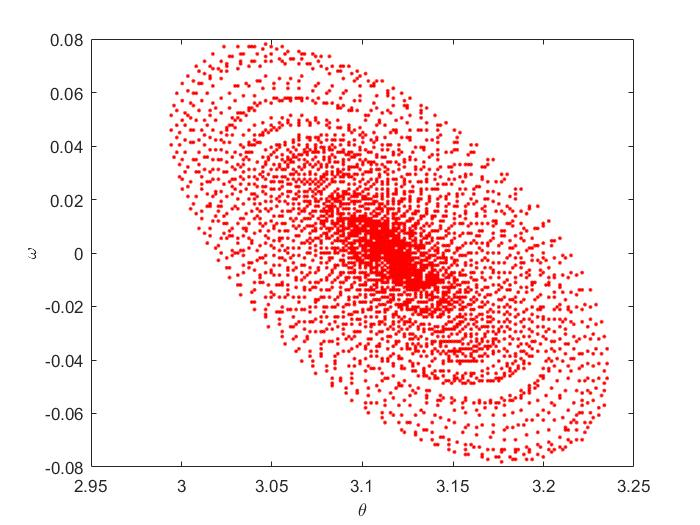
\includegraphics[scale=0.4]{images/prob1.jpg}
\captionof{figure}{state space plot}
\label{fig:prob1}
}
\end{minipage}

\section*{Problem 2}
\begin{enumerate}[label=(\alph*)]
\item 
The figure \ref{fig:prob2a} represents the reconstructed state plot on data2 using $\tau$ = 0.15 and m=7. The plot below looks likes a chaotic attractor.\\
\begin{minipage}{\linewidth}
{
\centering 
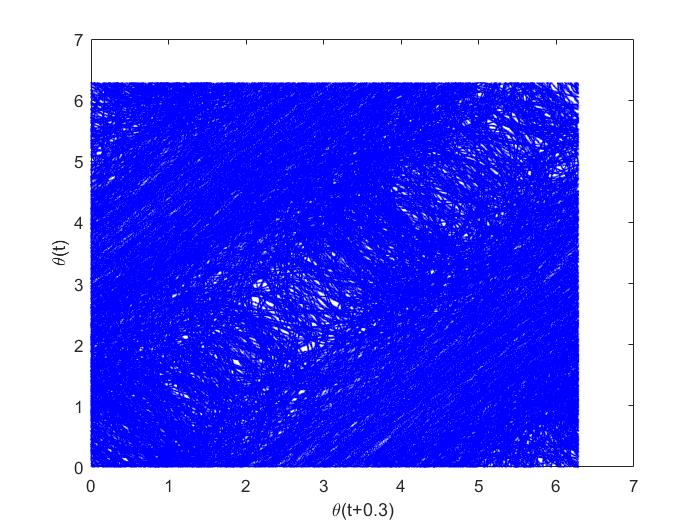
\includegraphics[scale=0.4]{images/prob2a.jpg}
\captionof{figure}{reconstructed state space plot}
\label{fig:prob2a}
}
\end{minipage}

\item
The below figure represents the reconstructed state plot on data3 using m=7 and raising $\tau$ from 0.01 to 1.5 secs. The plots below looks like a periodic attractor switching between two regions. We could see from the below plots becoming sparser as the $\tau$ value is increased, and two periods region size grows and shrinks. \\
\begin{minipage}{\linewidth}
{
\begin{table}[H]
\centering
\begin{tabular}{|c|c|}
	\hline
	\addheight{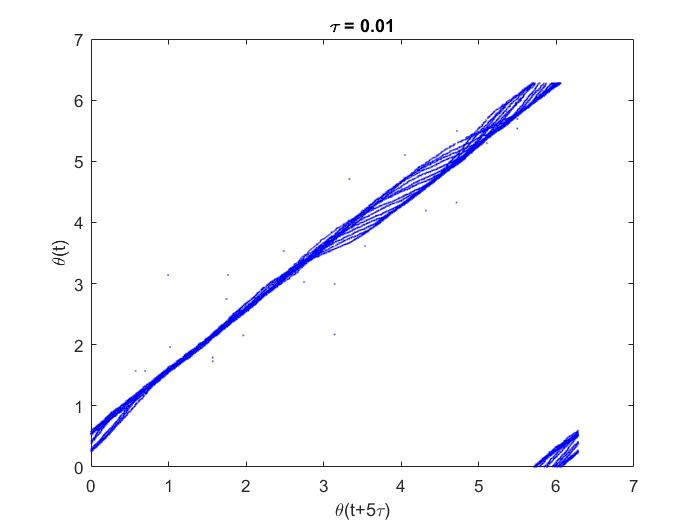
\includegraphics[width=75mm]{images/prob2b1.jpg}} &
    \addheight{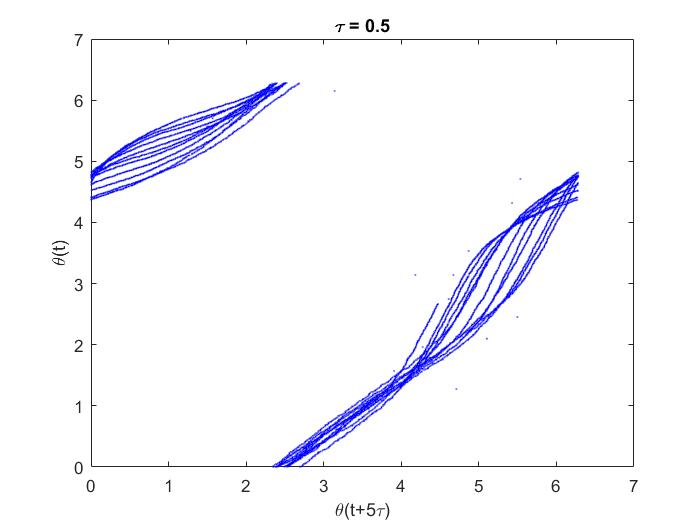
\includegraphics[width=75mm]{images/prob2b2.jpg}} \\
    \hline
    \addheight{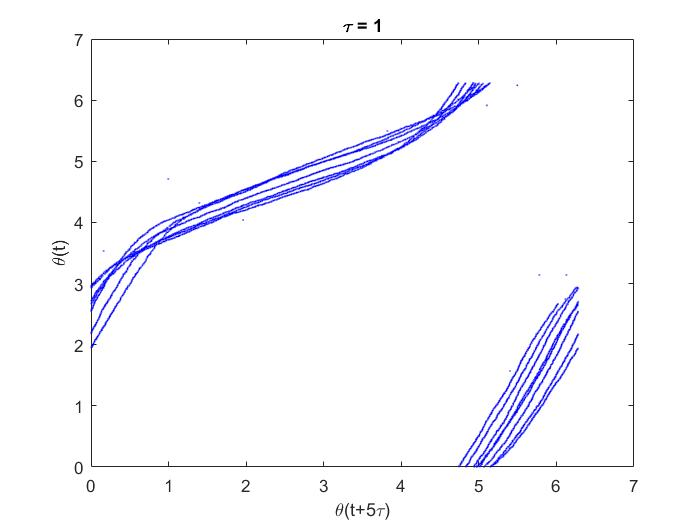
\includegraphics[width=75mm]{images/prob2b3.jpg}} &
    \addheight{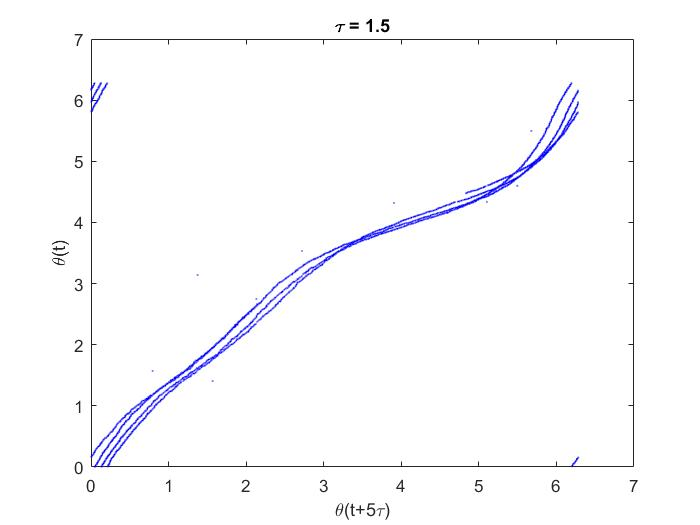
\includegraphics[width=75mm]{images/prob2b4.jpg}} \\
    \hline
\end{tabular}
\end{table}
}
\end{minipage}
\end{enumerate}

\section*{Problem 3}
\begin{enumerate}[label=(\alph*)]
\item
According to Taken's theorem $m > 2d$. To characterize a driven pendulum the dimension required is 3, whereas for a undriven pendulum the dimension required is 2, so by taken's theorem $m > 6$ for driven and $m > 4$ for undriven pendulum, in order to achieve successful embedding. 
\item
When m=2 the condition necessary to reconstruct a chaotic dynamical system from a sequence of observation of the state of a dynamical system is not sufficient according to Taken's theorem, as we will need atleast m = 7. Having m=25 is of no use as the dynamics of the reconstructed vector becomes deterministic way before, and the value of m preferred is atmost 2d+1 or sometimes even less.
\item
When $\tau = 10^{-16}$ the teeth of the comb used to reconstruct will be very close and some of the dynamics behavior will be missed as $\theta(t) = \theta(t+i\tau)$ will be more or less the same, and we will be seeing kind of a straight line. Whereas when $\tau = 10^{6}$ the teeth distance would be very high  and we will just seeing some random points in the picture that too only if the sample size is greater than $10^{6}$.
\end{enumerate}
\newpage
\section*{Problem 4}
\paragraph{•}
Using the TISEAN package to estimate $\tau$ parameter, I first ran the mutual tool with its default values. The default "max time delay" parameter was 20, and wasn't able to clearly find the first minimum in this curve.
\par\medskip
Then I played a little with "max time delay" parameter , and increased it's value till 750, to be sure that I have got the first minimum of the curve. I found the min at the sample interval 301 which equals 0.602 secs as the sample are taken every 0.002 secs. Below is the plot of $\tau$ vs mutual information. The mutual call I made to produce the data,
$$\textbf{mutual -D 1000 data2.first250sec -o out.dat} $$ 
\begin{minipage}{\linewidth}
{
\centering 
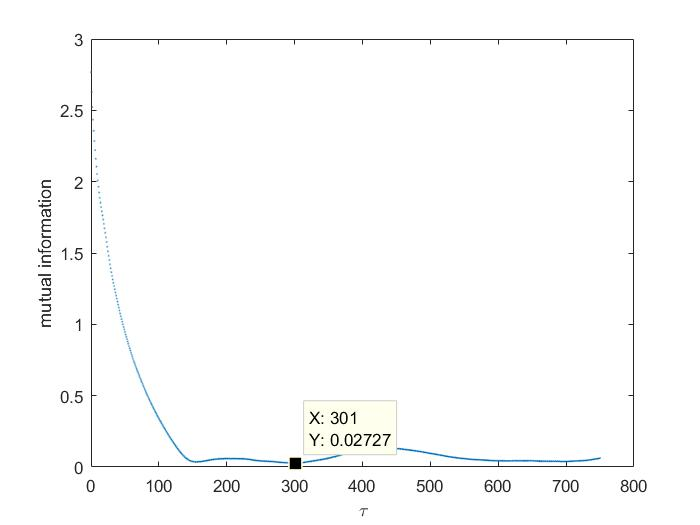
\includegraphics[scale=0.45]{images/prob4.jpg}
\captionof{figure}{$\tau$ vs mutual information}
\label{fig:prob4}
}
\end{minipage}

\section*{Problem 5}
In order to find a good value for embedding dimension m, I used TISEAN package false\_nearest tool. I found that good value of m = 8, as it is first value of m whose ratio of false\_neighbours went below 10\%. Below is the plot of m vs ratio of false\_neighbours. The call I made to produce the data.
$$\textbf{false\_nearest -M 1,10 -d 75 data2.first250sec -o out.dat}$$
\begin{minipage}{\linewidth}
{
\centering 
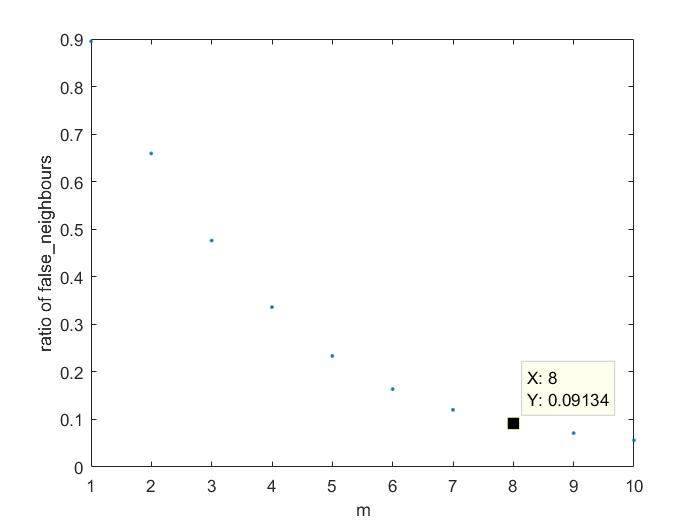
\includegraphics[scale=0.45]{images/prob5.jpg}
\captionof{figure}{m vs ratio of false\_neighours}
\label{fig:prob5}
}
\end{minipage}

\end{document}
